\chapter{Literature Review}
\label{cha:Literature Review}

\section{Car Following Models}
\label{sec:Car Following Models}
Most lane changing models stem from 'car-following models', which define actions for a vehicle based on the behaviour of its predecessors (the vehicles in front of it). One early car-following model was defined in 1981 by P.G. Gipps \citep{Gipps1981}. It was designed to mimic real-world driver behaviour, calculating a safe travel speed for a vehicle based on the speed of its predecessor. A safe travel speed is defined as a speed at which the driver can safely stop if the preceding driver stops.

Gipps' paper defines two equations, which provide constraints on the speed of vehicle $n$ at time $t + \tau$. $t$ is the current time and $\tau$ is the apparent reaction time, a constant for all vehicles. The first equation defines the acceleration constraint of the vehicle. It was obtained using measurements from an instrumented car.

\begin{equation}\label{Gipps1981Accel}
v_n(t+\tau) \leqslant v_n(t) + 2.5a_n\tau\Biggl(\frac{1 - v_n(t)}{V_n}\Biggr)\Biggl(\frac{0.025 + v_n(t)}{V_n}\Biggr)^{1/2}
\end{equation}

$v_n(t)$ is the speed of vehicle $n$ at time $t$. $a_n$ is the maximum acceleration the driver of vehicle $n$ wishes to undertake. $V_n$ is the target speed for vehicle $n$. The equation shows that the driver accelerates until close to their target speed. They then reduce their acceleration until it reaches zero. At this point the vehicle should be travelling at it's target speed.

The second constraint is the braking profile of the vehicle. This is given as

\begin{equation}\label{Gipps1981Brake}
\begin{split}
&v_n(t+\tau) \leqslant \\
&b_n\tau + \sqrt{\Biggl(b_n^2\tau^2 - b_n\biggl(2\Bigl[x_{n-1}(t) - s_{n-1} - x_n(t)\Bigr] - v_n(t)\tau - \frac{v_{n-1}(t)^2}{\hat{b}}\biggr)\Biggr)}
\end{split}
\end{equation}

$b_n$ is the most severe braking the driver of vehicle $n$ wishes to undertake. It is always a negative value, and should be considered negative acceleration. $\hat{b}$ is the driver of vehicle $n$'s best guess at $b_{n-1}$ where $n-1$ is $n$'s predecessor. $x_n(t)$ is the location of the front of vehicle $n$ at time $t$. $s_n$ is the effective size of vehicle $n$. This is equal to the physical length of $n$, plus a margin $n$'s successor is not willing to enter, even when $n$ is at rest.

Therefore, at time $t + \tau$, assuming the driver travels as fast as is safe, and within the limitations of the vehicle, the speed is given by the minimum of these two equations.

\begin{equation}
v_n(t) = \min{(\eqref{Gipps1981Accel},\eqref{Gipps1981Brake})}
\end{equation}

This model works well at describing the behaviour of traffic. However, translating this work to autonomous vehicles poses a number of problems. Firstly, the work is based on the behaviour of real-world drivers in instrumented vehicles. This introduces human driver variables into the equations. An autonomous vehicle with perfect sensors would have an almost negligible $\tau$, as the vehicles would have a very minimal reaction time. $s_n$ would also need to be adjusted. The margin added can be much less, as autonomous vehicles would be more precise than human drivers, driving closer to their predecessors. 

The model also ignores inter-vehicle communication. Autonomous vehicles could communicate their intentions to nearby vehicles, allowing them to act before they do. This could greatly reduce the following distance of successor vehicles, it would also allow vehicles to accelerate and move as a unit, or a 'platoon'. It would also allow autonomous vehicles to gain accurate value for $\hat{b}$.

In 2000 Treiber et al. suggested the 'Intelligent Driver Model' (IDM) \citep{Treiber2000}. In the IDM, the acceleration of vehicle $\alpha$, $\dot{v_\alpha}$, is defined using a continuous function of its velocity, $v_\alpha$; the distance to the rear of its predecessor, $s_\alpha$; and the velocity difference of $\alpha$ and it's predecessor, also known as the approaching rate $\Delta v_\alpha$. The vehicle interactions are solely based on $\alpha$'s relative acceleration to its predecessor. The model only provides position information for a vehicle in relation to its predecessor, and it does not provide its velocity at a given time, as Gipps' model does. 

The IDM is broken into two components. The first describes the behaviour of a vehicle on a free road.

\begin{equation}
\dot{v_\alpha} = a^{(\alpha)}\Biggl[1 - \biggl(\frac{v_\alpha}{v_0^{(\alpha)}}\biggr)^\delta\Biggr]
\end{equation}

Here $a^{(\alpha)}$ is the maximum acceleration of vehicle $\alpha$ and $v_0^{\alpha}$ is the desired velocity of $\alpha$. $\delta$ is the acceleration exponent, which is typically 4. 

The second component describes the behaviour of a vehicle as it approaches its predecessor. 

\begin{equation}
\dot{v_\alpha} = - a^{(\alpha)}\biggl(\frac{s^*}{s_\alpha}\biggr)^2
\end{equation}

As the gap, $s_\alpha$, between $\alpha$ and it's predecessor, gets closer to the desired minimum gap $s^*$, $\alpha$ decelerates.

Interpolating the two components gives us the IDM. 

\begin{equation}
\dot{v_\alpha} = a^{\alpha}\Biggl[1 - \biggl(\frac{v_\alpha}{v_0^\alpha}\biggr)^\delta - \biggl(\frac{s^*(v_\alpha,\Delta v_\alpha)}{s_\alpha}\biggr)^2\Biggr]
\end{equation}

The desired minimum gap in the IDM varies dynamically with velocity and approaching rate. It is given by the following function.

\begin{equation}\label{IDMSpacingFunction}
s^*(v,\Delta v) = s_0^{(\alpha)} + s_1^{(\alpha)}\sqrt{\frac{v}{v_0^{(\alpha)}}} + T^\alpha v + \frac{v\Delta v}{2\sqrt{a^{(\alpha)}b^{(\alpha)}}}
\end{equation}

The equation takes the bumper-to-bumper space $s_0^{(\alpha)}$, also known as the minimum jam distance, and adds the comfortable jam distance $s_1^{(\alpha)}$. The bumper-to-bumper space is the minimum gap between $\alpha$ and its predecessor in stationary traffic. The comfortable jam distance is an extra distance added on for comfort, and to allow for a slower driver reaction time. In the paper, this value is set to $0$. We can also consider it negligible for autonomous vehicles. $T$ is the safe time headway; it represents the time required for the vehicle to safely come to a stop. Finally $b^{(\alpha)}$ is the desired deceleration for $\alpha$.

The IDM does not attempt to directly mimic human behaviour in traffic situations. It models a general acceleration and braking profile for a given vehicle. As such, it is well suited for adaptation by autonomous vehicle models, as seen in \citep{Kesting2007}. However, similarly to Gipps' model, the standard IDM only applies to single lane traffic. It also ignores inter-vehicle communication and platooning opportunities. 

In vehicle platoons, such as those analysed by Kamali in 2016 \citep{Kamali2016}, each vehicle autonomously follow it's predecessor, with the lead vehicle controlling the overall pace of the platoon. Platoons make heavy use of vehicle-to-vehicle (V2V) communication to allow vehicles to join and leave, as well as to continuously control vehicle spacing and velocity.

Kamali developed a model for an automated platoon, defining procedures for vehicles joining and leaving. 

A joining vehicle can integrate at either the back or the middle of the platoon. The vehicle first sends a join request to the platoon leader. If the vehicle is at the back of the platoon the leader sends an agreement and the vehicle follows its predecessor. If the vehicle requests to join in front of another platoon vehicle, the leader first asks the platoon vehicle to increase space; once the space is large enough for the joining vehicle, the leader sends an agreement. The joining vehicle then manoeuvres into the space and follows the preceding vehicle. Having now joined the platoon, the vehicle sends a confirmation to the leader. The leader then requests that the vehicle that gave way for the joining vehicle decreases their spacing back to normal.

A leaving vehicle sends a request to the leader. When it receives permission to leave the vehicle increases its spacing from its predecessor; once the vehicle is at its maximum distance from its predecessor the vehicle can change lanes. Once out of the convoy the vehicle sends an acknowledgement to the leader.

This model isn't very strict, acting as more of a set of requirements than a true model. The paper sets the requirements using pre-defined gaps, and has no strict calculations guiding following characteristics. It could be implemented using spacing rules from both the IDM and Gipps' model, however, by using V2V communication, the lead vehicle can control the actions of all vehicles in its platoon. Instead of using IDM or Gipps' model, the lead vehicle can control the gaps between vehicles so that they all increase and decrease simultaneously. The gaps could be based on the platoon's velocity, perhaps using \eqref{IDMSpacingFunction} from the IDM. By centralising control in this way, vehicle platoons can avoid the traffic shock effect \citep{Daganzo1994}.

\section{Centralised and Decentralised}
\label{sec:Centralised and Decentralised}

We can divide approaches to autonomous vehicles into centralised and decentralised solutions. Centralised solutions rely on an external agent to manage vehicles. Vehicles use vehicle-to-infrastructure (V2I) communication channels to send information and receive instructions from the external agent. Decentralised solutions use vehicle-to-vehicle (V2V) communication to let other vehicles know their state, their intentions and to arrange any complex actions that might affect surrounding vehicles.

\subsection{Centralised Systems}
\label{subsec:Centralised Systems}
The Autonomous Vehicle Intersection management system (AIM) described in \citep{Dresner2004} is an example of a centralised V2I system. The system works by dividing the intersection into a grid of $n \times n$ reservation tiles. Drivers 'call ahead' to the intersection sending information packets containing

\begin{enumerate}
\item The time the vehicle will arrive.
\item The velocity at which the vehicle will arrive
\item The direction the vehicle will be facing when it arrives
\item The vehicle's maximum velocity
\item The vehicle's maximum and minimum acceleration
\item The vehicle's length and width
\end{enumerate}

The intersection infrastructure simulates the journey of the vehicle through the intersection, noting the tiles occupied by the vehicle at each time interval. If any cell is reserved at the same time step the intersection rejects the request. The driver will start decelerating and continue making requests until it obtains a reservation. It will not enter the intersection without a reservation, even if that means coming to a stop at the intersection.

\begin{figure}[htb]
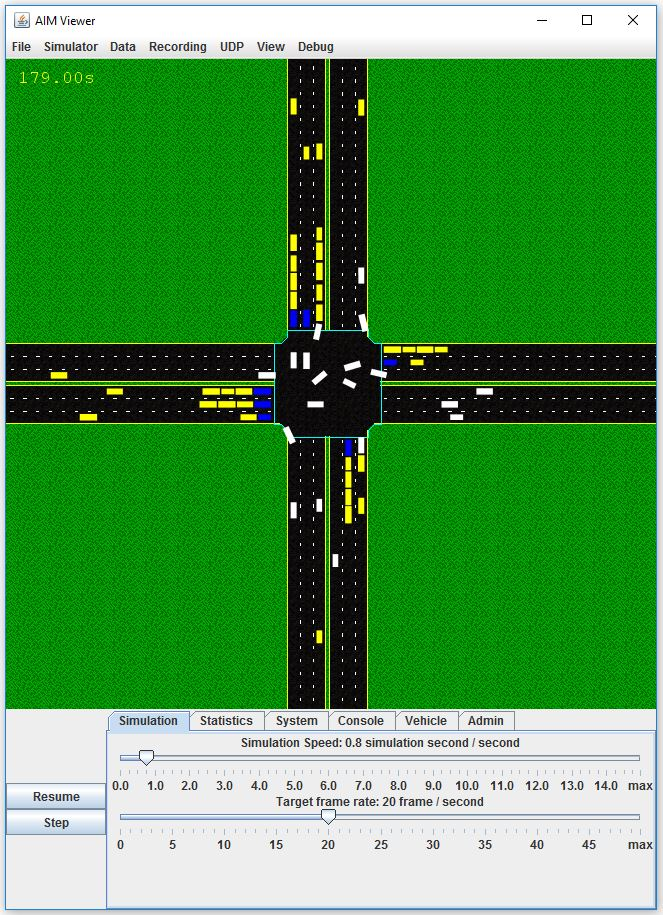
\includegraphics[width=\textwidth]{AIMOriginal.JPG}
\caption{Screenshot of the AIM Simulator}
\label{fig:AIMOriginal}
\end{figure}

A grid-based reservation system works well in high traffic zones like intersections, because it forces all vehicles to communicate with a single entity. This entity has a global-view of activity at the junction, allowing the system to make vehicle management decisions more easily. A V2V solution would require more complex communication protocols involving large numbers of vehicles. The volume of messages required for each vehicle to obtain a global view of the intersection would be considerably larger, and as such, most vehicles will never get a complete understanding of the status of the intersection.

A centralised system for lane changing was described in a paper by Atagoziyev et al. in 2016 \citep{Atagoziyev2016}. This system uses roadside infrastructure to help groups of vehicles change lanes before they reach a 'critical-position', such as a motorway exit or intersection. The vehicles send their position and velocity information to the roadside infrastructure; the system then sends a number of orders to the vehicles such that they safely rearrange themselves into the correct lanes.  Because the distance travelled by the vehicles involved can be large, particularly at high speeds, the system would struggle to use a reservation tile based system as AIM did, instead Atagoziyev's system manages the gaps between vehicles to safely relocate vehicles into the correct position. A more comprehensive overview is given in \ref{subsec:Lane Changing to hit a target lane}.

Atagoziyev's system would only need to be applied during the approach to critical-positions. Vehicles could be managed using platoons or another vehicle following model until that point. A centralised system provides a single communication point which manages all of the vehicles that want to change lanes. This helps to reduce the volume of communications required and creates an entity with a global view of the vehicles' positions and goals. A V2V solution would most likely require more communications and may never obtain a complete picture of the situation, possibly leading to sub-optimal lane changing orders.

Note that Atagoziyev's system could be adapted, such that all of the vehicles communicate with the platoon leader instead of roadside infrastructure. Though this could be called a V2V communication solution, the effective solution is still considered centralised, as all decisions are made by one entity.

\subsection{Decentralised Systems}
\label{subsec:Decentralised Systems}
The main arguments against centralised systems generally tend to stem from concerns over feasibility and fault tolerance. A centralised V2I solution relies on one system always being available to manage vehicles. The original implementation of the AIM system works well, but if the system were to fail and no longer provide reservations then approaching vehicles will simply halt at the intersection. In a worst case scenario, the system would still give reservations, but fail to compare them to reservations already in place, causing major car crashes in the intersection. Having, a single point of failure (SPOF) like this is a major concern, particularly when lives are on the line.

A paper by Van Middlesworth et al. in 2008 \citep{VanMiddlesworth2008} defined a decentralised version of the AIM model using V2V communication protocols. 

In Van Middlesworth model each vehicle can broadcast two different types of message. These messages are broadcast repeatedly with a specified period.
\begin{enumerate}
\item CLAIM
This is a message indicating the vehicle's intention to traverse the intersection. It provides the vehicle's VIN, arrival lane, turning direction, arrival time and exit time. It also provides a message id, which increments when a new message is broadcast. Finally, the CLAIM message contains a boolean indicating whether the vehicle has stopped at the intersection.
\item CANCEL
This message releases any currently held reservation, it contains the vehicle's VIN and a message id, which acts the same as the message id in CLAIM.
\end{enumerate}

Two CLAIM messages are in conflict if their paths, as determined by their lane and turn parameters, are incompatible and their time intervals, as determined by their arrival and exit times, overlap. To resolve the conflict Van Middlesworth defines a priority ordering over claim messages using the following rules:
\begin{enumerate}
\item If neither vehicle is stopped at the intersection, the claim with the earliest exit time has priority.
\item If both vehicles are stopped, the vehicle whose lane is 'on the right' has priority. This is defined similarly to current US 4-way stop rules.
\item If neither lane can be considered to be on the right the vehicle who is not making a turn has priority.
\item If no other priority order can be established, the vehicle with the lowest VIN has priority.
\end{enumerate}

The protocol starts with approaching vehicles receiving messages from existing pending vehicles. An approaching vehicle may not start broadcasting it's own messages until it is within 'lurk distance' of the intersection. 

Once within lurk distance the vehicle tries to make a reservation using a CLAIM message. The vehicle will continue generating CLAIM messages, searching for an available time block, increasing and decreasing its velocity as necessary, until it finds one that allows it to traverse the intersection without any other CLAIM having priority over it.

Once the vehicle has a CLAIM broadcasting it may need to change it if it's looking like the vehicle might be late to the intersection or if a competing CLAIM arrives with a higher priority. A vehicle might also change its CLAIM to take advantage of a newly available time slot. In this situation the vehicle must then send a CANCEL message and a new CLAIM. Once the vehicle reaches the intersection it must traverse according to its current CLAIM, broadcasting its CLAIM throughout the traversal. At this point, the vehicle has the highest priority CLAIM and cannot be interrupted.

The main drive behind the unmanaged AIM intersection was to reduce cost. Adding in new infrastructure to an intersection costs money, and it might not be considered worthwhile for small intersections with only one or two lanes on each side. An unmanaged, decentralised system like that described by Van Middlesworth would drastically reduce the cost to the state in creating automated road networks.

Cost also becomes a major issue for centralised systems when you consider fast moving situations such as lane changing on a motorway. To implement Atagoziyev's model, vehicles must remain in range of the roadside infrastructure. This would mean that the infrastructure will have to continue on for a long distance, which could become very expensive, especially given the number of critical-positions on a motorway. Decentralised solutions reduce these costs massively.

Two examples of decentralised lane changing models are Gipps' 1986 driver decision model \citep{Gipps1986} and the MOBIL model developed by Kesting et al. in 2007 \citep{Kesting2007}. These models are decentralised and as such do not have to rely on roadside infrastructure in order to change lanes. This greatly reduces the cost of both implementations and allows the vehicles to be more flexible as to when they change lanes, no longer having to wait until they reach the lead up to a critical-position supported by roadside infrastructure. This flexibility means that vehicles could change lanes to increase their average velocity rather than just changing lanes in order to make a turn or leave the motorway at a critical-position. It also allows vehicles to deal with unexpected situations far from any roadside infrastructure. For example, a broken down car blocking a lane can be evaded. There is more information on Gipps' 1986 model and MOBIL in \ref{sec:Making lane changing decisions}.

\section{Making lane changing decisions}
\label{sec:Making lane changing decisions}
There are a number of reasons that a driver would want to change lanes. The most obvious being that the journey the driver wishes to complete requires the vehicle to move into a different lane. In this case the vehicle \emph{must} change lanes before it reaches a critical position. Beyond this position the driver will need to change their planned route, most likely extending their journey time. 

Another reason a driver might change lanes is in order to increase velocity, with the aim of reducing journey time. In general, a driver will aim to change lanes if their average velocity in their current lane is much less than that the velocity it could be achieving in another lane.

\subsection{Lane Changing to hit a target lane}
\label{subsec:Lane Changing to hit a target lane}
In 1986 Gipps' modelled driver behaviour in real world circumstances, characterising the decisions a driver has to make in order to determine whether to change lanes \citep{Gipps1986}. The paper was designed to be used with the Gipps' 1981 car-following model \citep{Gipps1981}, explained in \ref{sec:Car Following Models}.

The model itself is constructed as a flow chart, in which the decision nodes are the choices a driver must make.You can see the flowchart in Figure \ref{fig:Gipps1986Flowchart}.

\begin{figure}[htb]
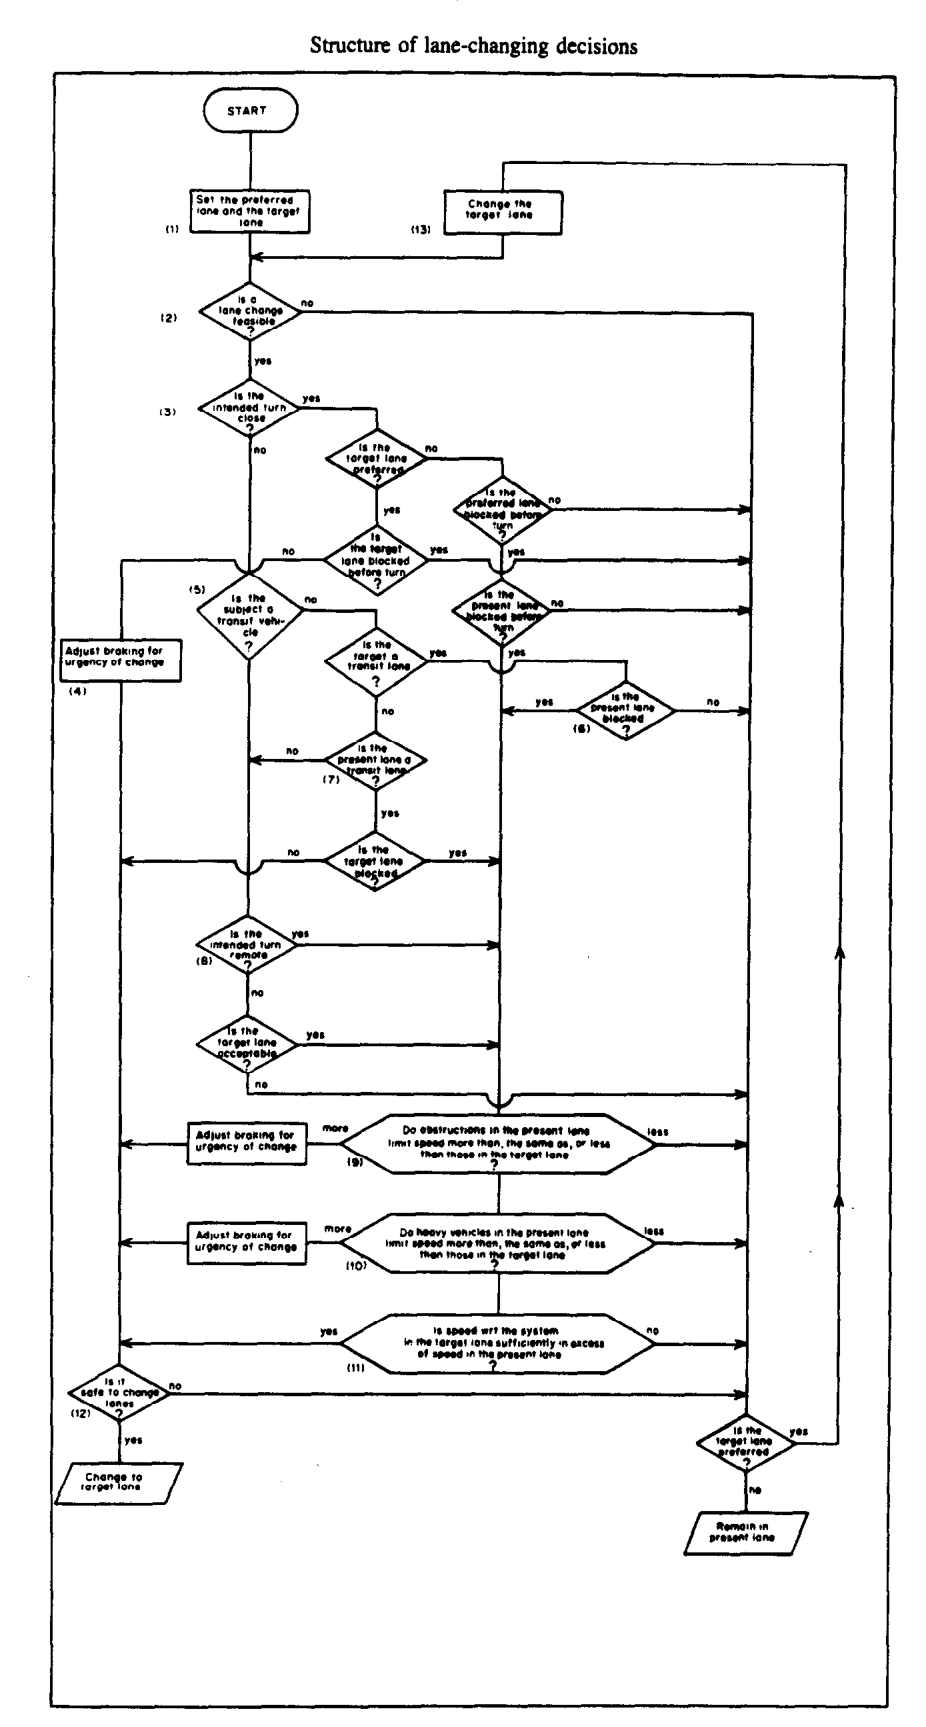
\includegraphics[width=\textwidth]{Gipps1986Flowchart.png}
\caption{The flowchart for lane changing decisions from \citep{Gipps1986}}
\label{fig:Gipps1986Flowchart}
\end{figure}

After determining whether a lane change is feasible the model considers whether the driver needs to move into another lane because they are heading towards a critical point.

These decisions are modelled in nodes 3 and 4.

\begin{enumerate}
\item[3] \textit{Driver behaviour close to the intended turn}

If the driver is close to their intended turn then they will always attempt to change into their preferred lane. Only if blocked will they consider moving into another lane. 

'Close' varies depending on regional differences and the level of traffic, but in the model, close is defined as the driver being within a distance equal to ten seconds of travel from the turn at the driver's desired speed.

\item[4] \textit{Urgency of changing lanes}

The urgency of changing lanes increases as the driver gets closer to their turn. The willingness of the driver to brake harder and accept smaller gaps increases as the driver gets closer to their intended turn.

In the implementation, the braking rate a driver is willing to when first becoming close doubles by the time the intended turn is reached. 

\begin{itemize}
\item[$D_n$] is the location of the intended turn
\item[$V_n$] is the desired (or free) speed of the driver
\item[$b_n^*$] is the most severe braking the driver would otherwise be willing to undertake
\end{itemize}

\begin{equation}
b_n = \Biggl[2 - V_n\frac{(D_n - x_n(t))}{10}\Biggr]b_n^*
\end{equation}

\end{enumerate}

Similarly to Gipps 1981 car-following model, this driver decision model is based on human driver behaviour and as such falls into similar pitfalls. There could be more optimal driver behaviours which would ensure that a driver is in the correct lane well before the critical position. However, because Gipps 1986 model is designed to model human driving behaviour we can expect it to perform less than optimally.

Atagoziyev's model is designed around autonomous vehicles, which allows it to take advantage of vehicle-to-vehicle communication. The model manages a set of vehicles over two lanes, organising their movements into their preferred lanes before they reach a critical position.

To do this the model keeps track of the gaps between vehicles and their relative speeds using roadside infrastructure. Then, a series of equations, each describing a different situation, are used to determine the behaviour of the vehicle.

In the paper SV (subject vehicle) refers to the vehicle that wants to change lanes. CL (current lane) is the vehicle in front of the SV. TL (target lane) is the vehicle the SV wants to be behind in its target lane. LV (lag vehicle) is the vehicle that will be behind SV once it moves to its target  lane. Atagoziyev defines seven equations for manipulating vehicles between lanes. They are used in different contexts, each based on the relative positions of the surrounding vehicles. The contexts for each equation are given below, along with the behaviour from the equation during that context.

\begin{enumerate}
\item[Case 1] \textit{SV too close to CL in its current lane or TL if it changed lanes.}

SV slows down until the gap is sufficiently large enough.
\item[Case 2] \textit{SV has a large gap between itself and TL and CL, however, LV is too close to SV}

SV can approach CL and TL as long as the gap remains large enough. LV needs to open up a sufficient gap behind SV.
\item[Case 3] \textit{SV has the minimum allowable gap to TL and CL, but LV is too close}

SV follows the closest leader and waits until LV creates the necessary gap.
\item[Case 4] \textit{The gaps between SV and CL/TL/LV are sufficient. But CL/TL are not travelling at the 'nominal speed' established for all vehicles in this exchange}

SV maintains a sufficient gap, waiting for CL/TL to travel at nominal speed again.
\item[Case 5] \textit{SV and CL/TL/LV have sufficient gaps and CL/TL are travelling at nominal speed.}

SV performs the lane change, maintaining nominal speed.
\item[Case 6] \textit{SV obtains the minimum gap to CL/TL and LV maintains a sufficient gap. CL/TL are not travelling at nominal speed}

SV maintains the minimum gap, waiting for CL/TL to travel at nominal speed again.
\item[Case 7] \textit{SV obtains the minimum gap to CL/TL and LV maintains a sufficient gap. CL/TL are travelling at nominal speed}

SV performs the lane change, maintaining nominal speed.
\end{enumerate}

These equations are the building blocks that lead to a lane change. The flowchart in Figure \ref{fig:AtogoziyevFlowchart} shows how they work together to enact a single lane change.

\begin{figure}[htb]
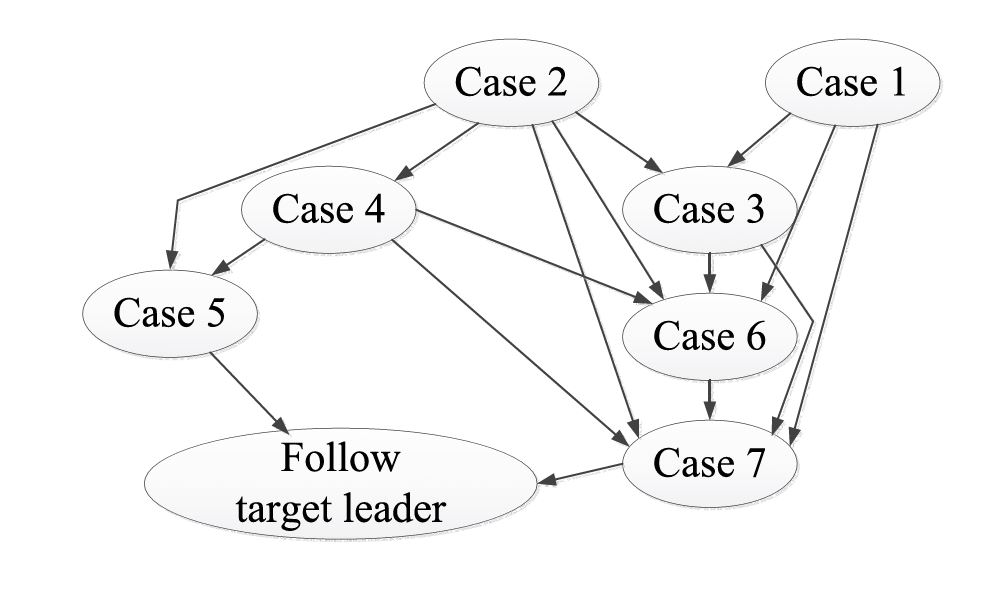
\includegraphics[width=\textwidth]{AtagoziyevFlowchart.JPG}
\caption{The flowchart for Atagoziyev's Lane Changing model equations}
\label{fig:AtogoziyevFlowchart}
\end{figure}

Using this algorithm, we can move multiple vehicles into their correct lanes. LV always provides space to allow each changing vehicle into the correct lane. All of the vehicles are working with each together, such that they can all reach their goal. Comparing this to Gipps' 1986 model, where drivers are acting solely in their own interest, we can see that by having an external agent managing lane changes, the autonomous vehicles can achieve results that might not be possible in situations where drivers are acting selfishly. For example, in a grid locked situation, drivers following Gipps' model might never be able to move into their desired lane; however vehicles following Atagoziyev's model would open up spaces allowing vehicles to move through the traffic.

\subsection{Lane Changing to improve overall velocity}
\label{subsec:Lane Changing to improve overall velocity}
Gipps' driver decisions model also considered situations where the driver does not have to be in any particular lane. The model considers the effects of transit lanes, heavy vehicles and the effect of the preceding vehicle on the driver's vehicle. These are shown in nodes 5 to 7 and 9 to 11 of Gipps' flowchart in Figure \ref{fig:Gipps1986Flowchart}.

\begin{enumerate}
\item[5] \textit{Transit vehicles and lanes}
Transit lanes are lanes dedicated solely for public transport and other high occupancy vehicles. These include vehicles such as buses, taxis and carpool cars. These vehicles are known in the model as 'transit vehicles'.
\item[6] \textit{Entry of nontransit vehicles into transit lanes}
If there is an obstruction in the present lane, it is often considered to be a valid reason for a non-transit vehicle to enter a transit lane. 
\item[7] \textit{Departure of nontransit vehicles from a transit lane}
Once the obstruction has been cleared, nontransit vehicle must move back into a valid lane. This forced departure does not affect vehicles that are close to their intended turn.
\item[9] \textit{Relative advantages of present and target lanes}
If the driver has not yet been forced to change lanes by any other factors, then they can look at the relative advantages of the present and target lanes, considering obstructions and then determining which lanes obstructions will have the least effect on their safe speed.
\item[10] \textit{The effect of heavy vehicles} 
If obstructions are level with each other or beyond the range a driver considers, then the driver considers the next heavy vehicle in each lane, as if it were the leading vehicle in an ordinary car following situation. The driver then selects the lane which will give them the higher speed.
\item[11] \textit{The effect of the preceding vehicle}
If there are then no heavy vehicles, the driver considers the speed possible in each lane and then changes if they gain a 'sufficient' speed advantage. This is again, subjective, depending on the present lane, target lane and the type of vehicle.
\end{enumerate}

Again, Gipps' 1986 model was built with human drivers in mind, and as such it fails to take advantage of the benefits of autonomous vehicles such as platooning and vehicle-to-vehicle communications.

Work by Kesting et al. in 2007 \citep{Kesting2007} describes a decentralised model of lane changing that lets vehicles change lanes to increase velocity whilst still ensuring that the overall traffic flow is not disrupted. This helps to avoid traffic shocks and maintains smooth traffic flow. In order to do this, Kesting introduces the MOBIL or 'Minimising Overall Braking Induced by Lane Changes' model. The model uses two criterion that the vehicle must satisfy.

The first criterion deals with safety, ensuring that the deceleration of a successor vehicle $\tilde{a}_n$ in the target lane doesn't exceed a safety limit $b_{safe}$.

\begin{equation}
\tilde{a}_n \geq -b_{safe}
\end{equation}

This criterion effectively puts a limit on the level of braking a vehicle changing lanes can cause another vehicle to undergo if it pulls out in front of it.

The second criterion is the 'incentive criterion' which is what motivates a driver to change lanes. This criterion introduces a 'politeness factor' $p$ which expresses the extent to which nearby vehicles affect a driver's lane changing decision. 

The paper discusses the differences between symmetric ('US') lane changing rules and asymmetric ('European') passing rules, however in this paper we only use US lane changing rules. This gives the incentive criterion:

\begin{equation}
\underbrace{\tilde{a}_c - a_c}_\text{driver} + p(\underbrace{\tilde{a}_n  - a_n}_\text{new follower} + \underbrace{\tilde{a}_o - a_o}_\text{old follower}) > \Delta a_{th}
\end{equation}

$\tilde{a}_x - a_x$ is the utility a driver x gets due to the lane change, where $\tilde{a}_x$ is the acceleration of vehicle x after the lane change and $a_x$ was their acceleration before the lane change. $c$ is the vehicle changing lanes, $n$ is the vehicle behind $c$ once it changes lanes, and $o$ is the vehicle following $c$ before the lane change. $\Delta a_{th}$ is the threshold at which the driver will change lanes. It is designed to model inertia. A driver won't change lanes unless they get above a specific utility gain. The politeness factor $p$ varies from $0$ to $1$, where $p = 0$ is the most selfish behaviour and $p = 1$ describe drivers who won't change lanes unless collectively all of the drivers gain a utility greater than the threshold. When $p > 1$ drivers won't change lanes at all if it negatively affects the surrounding traffic, drivers will even go so far as to execute lane changes which reduce their own utility. Likewise drivers with $p < 0$ will go out of their way to negatively affect other drivers, even reducing their own utility to do so.

The idea of a MOBIL model means that drivers will only change when it increases the sum of all of the accelerations increases. This would be at $p = 1$ and $\Delta a_{th} = 0$. In this case the equation becomes 

\begin{equation}
\tilde{a}_c + \tilde{a}_n + \tilde{a}_o > a_c + a_n + a_o 
\end{equation}

Kesting found that the most important parameter affecting the rate of lane changing was $p$. With a $p$ value of 1 the maximum lane changing rate was almost halved. Kesting also discovered that 'altruistic' lane changing behaviour increased the mean speed of both lanes involved in the simulation, improving overall traffic performance.

Comparing this to Gipps' 1986 approach we can see that MOBIL is far more considerate of other drivers and as such the overall speed of the vehicles on the road could be higher. MOBIL is also designed for autonomous vehicles, which allows it to enforce 'altruistic' behaviour from vehicles on the road. The model could also be extended to include V2V communications. Transmitting accurate braking profiles to other vehicles would make it easier to determine the effect a lane change would have on the overall system.